\begin{frame}
\frametitle{Folds}
\begin{block}{Left, Right, FileNotFound}
\begin{itemize}
\item<1-> You may have heard of \emph{right folds} and \emph{left folds}
\item<2-> Haskell: \lstinline{foldr}, \lstinline{foldl}
\item<2-> Scala: \lstinline{foldRight}, \lstinline{foldLeft}
\item<2-> C\# (BCL): \emph{no right fold}, \lstinline{Aggregate} \emph{kind of} 
\item<2-> C\# (xsharpx): \lstinline{FoldRight}, \lstinline{FoldLeft} 
\end{itemize}
\end{block}
\end{frame}

\begin{frame}
\frametitle{Folds}
\begin{block}{Developing intuition for folds}
\begin{itemize}
\item<1-> When do I know to use a fold?
\item<2-> When do I know which fold to use?
\item<3-> What do the fold functions \emph{actually do}?
\end{itemize}
\end{block}
\end{frame}

\begin{frame}
\frametitle{Developing intuition for folds}
\begin{block}{There is much effort toward answering these questions}
\begin{figure}
\centering
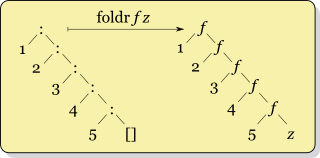
\includegraphics[width=0.5\textwidth]{image/Right-fold-transformation.png}
\caption{right fold diagram}
\end{figure}
\end{block}
\end{frame}

\begin{frame}
\frametitle{Developing intuition for folds}
\begin{block}{There is much effort toward answering these questions}
\begin{figure}
\centering
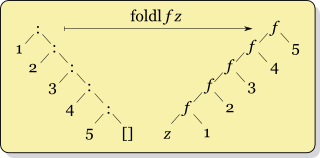
\includegraphics[width=0.5\textwidth]{image/Left-fold-transformation.png}
\caption{left fold diagram}
\end{figure}
\end{block}
\end{frame}

\begin{frame}
\frametitle{Developing intuition for folds}
\begin{block}{and terse explanations}
\begin{itemize}
\item<1-> the right fold does folding from the right and left fold, folding from the left
\item<2-> choose the right fold when you need to work with an infinite list 
\end{itemize}
\end{block}
\end{frame}

\begin{frame}[fragile]
\frametitle{Developing intuition for folds}
\begin{block}{Unfortunately}
\begin{center}
most of these are misrepresentative, incomplete, or wrong
\end{center}
\end{block}
\end{frame}

\begin{frame}
\frametitle{Goals}
\begin{block}{Goals for today}
\begin{itemize}
\item Develop a robust and accurate description and intuition for each list fold function
\item Ask and answer practical questions, given this intuition
\end{itemize}
\end{block}
\end{frame}

\begin{frame}
\frametitle{Goals}
\begin{block}{First things first}
\center
In practice, the \lstinline[basicstyle=\ttfamily]$foldl$ and \lstinline[basicstyle=\ttfamily]$foldr$ functions are \textbf{very different}.
\end{block}
So let us think about and discuss each separately.
\end{frame}

